\documentclass[10pt]{beamer}

\mode<presentation>
{
  \usetheme[height=1.25cm]{Madrid}
  \setbeamertemplate{navigation symbols}{}
  \setbeamercolor{alerted text}{fg=illini}
}
\usebackgroundtemplate{
\includegraphics[width=\paperwidth,height=\paperheight]{uc-background}}

\usepackage[english]{babel}
\usepackage{epsfig,subfigure,bm}
\usepackage{multimedia}
\usepackage{psfrag}
\usepackage{animate}

%%%%%% Begin of my macros and options

\setbeamertemplate{section in toc shaded}[default][55]
\setbeamertemplate{subsection in toc shaded}[default][55]
\setbeamercolor{block title}{fg=white,bg=illini}
\setbeamercolor{block body}{fg=black,bg=mygrey}

\setbeamercolor{emphprimary}{fg=CBlue}
\setbeamercolor{emphsecondary}{fg=illini}
\setbeamercolor{emphtertiary}{fg=mygreen}
\definecolor{darkForestGreen}{rgb}{.1,1,.1}
\definecolor{veryLightGray}{rgb}{.9,.9,.9}
\definecolor{greenApple}{rgb}{.3,.9,.3}

\setbeamercolor{frametitle}{bg=CBlue}
\setbeamercolor{title}{bg=CBlue}

\usepackage{amsmath,amssymb,amsxtra,amsthm}
\usepackage{algorithm,algorithmic}
\usepackage{natbib}
\usepackage{bibentry}
\usepackage{xspace}
\usepackage{changepage}

\pdfmapfile{+sansmathaccent.map}

\definecolor{myblue}{rgb}{.2,.2,.7}
\definecolor{myred}{rgb}{.7,.2,.2}
\definecolor{mygreen}{rgb}{.2,.7,.2}
\definecolor{mygrey}{rgb}{0.9,0.9,0.9}
\definecolor{CBlue}{cmyk}{1,0.25,0,0}
\definecolor{illini}{rgb}{0.98,0.4,0.05}
\definecolor{black}{cmyk}{0,0,0,1}

\newcommand{\myemph}[1]{{\usebeamercolor[fg]{emphprimary}
    \textbf{#1}}}
\newcommand{\myemphalt}[1]{{\usebeamercolor[fg]{emphsecondary}
    \textbf{#1}}}

\graphicspath{{figs/}}

\title[Math for Robotics] % (optional, use only with long paper titles)
{CSE276C - Interpolation and Approximation}

\author[H.~I. Christensen] % (optional, use only with lots of authors)
{Henrik I.~Christensen}
% - Give the names in the same order as the appear in the paper.  -
% Use the \inst{?} command only if the authors have different
% affiliation.

\AtBeginSection[]
{
   \begin{frame}
       \frametitle{Outline}
       \tableofcontents[currentsection]
   \end{frame}
}

\institute[UCSD] % (optional, but mostly needed)
{
  \begin{minipage}[c]{.2\textwidth}
    
\includegraphics[width=.65\linewidth]{ucsealnew}%
  \end{minipage}%
  \begin{minipage}[c]{.6\textwidth}
    \small
%%    \begin{center}
      Computer Science and Engineering\\
      University of California, San Diego\\
      \myemph{\url{http://cri.ucsd.edu}}\\          
%%    \end{center}

  \end{minipage}
%%  \vspace*{1ex}
}
%% - Use the \inst command only if there are several affiliations.
%% - Keep it simple, no one is interested in your street address.

\bigskip

\date[Oct 2024]% (optional, should be abbreviation of conference name)
{\small October 2024}

\begin{document}
  
\nobibliography{/Users/hic/Dropbox/bibliography/bib-file}
\bibliographystyle{plain}


\begin{frame}[plain]
  \titlepage
\end{frame}

\section{Introduction}


\begin{frame}
  \frametitle{Material}
  \begin{itemize}
  \item Numerical Recipes: Chapter 3
  \item Math for ML: Chapter 9
  \end{itemize}
\end{frame}

\begin{frame}
  \frametitle{Objective}
  \begin{itemize}
  \item How can we find an approximation / interpolation based on a set of data points?
    \pause
  \item Model Based
    \begin{itemize}
    \item We have domain knowledge that can be used:
    \item Battery recharge
    \item Dynamic Model of Drive System
    \item Material properties for grasping
    \end{itemize}
  \item Data Driven
    \begin{itemize}
    \item All we have is the data (and possible constraints)
    \item Driving in traffic, Painting, ...
    \end{itemize}
  \end{itemize}
\end{frame}

\begin{frame}
  \frametitle{Example}
  \centerline{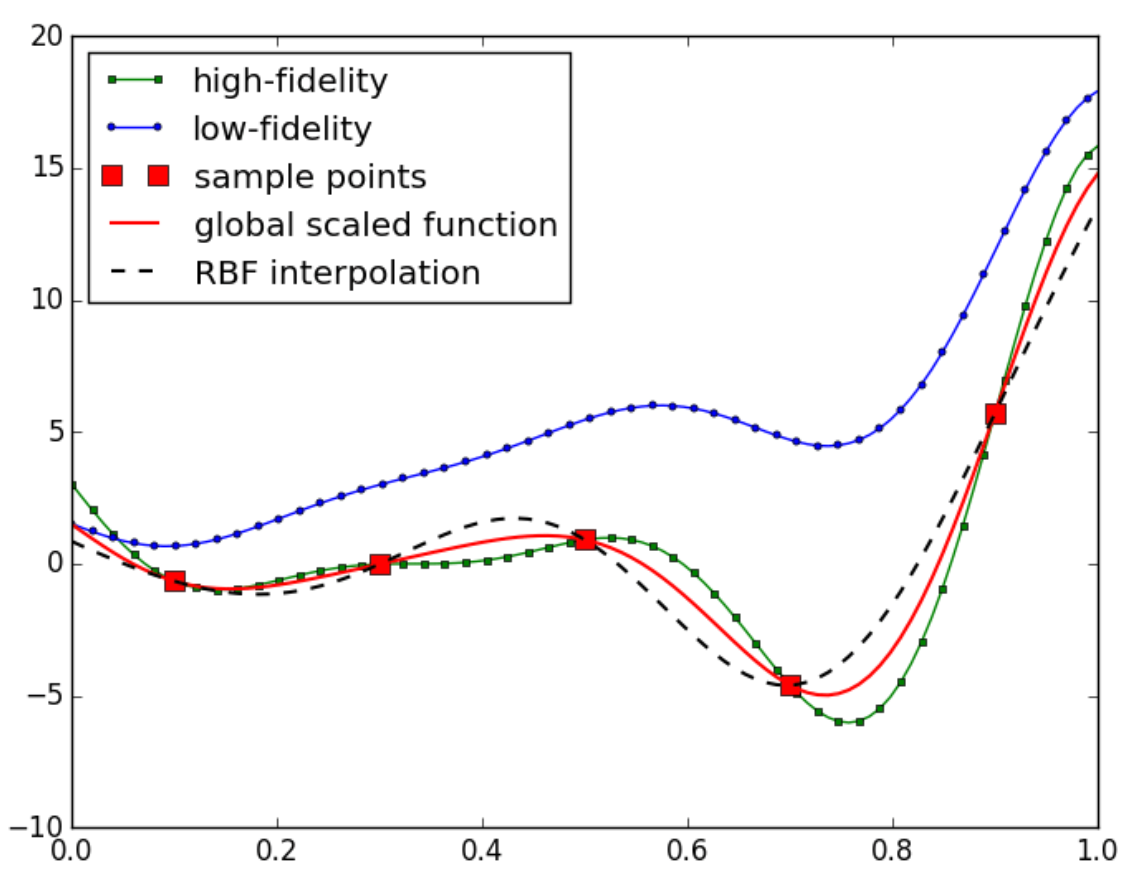
\includegraphics[height=7cm]{approximation-methods.png}}
\end{frame}

\begin{frame}
  \frametitle{Weierstrass Approximation Theorem}
  \begin{block}{Weierstrass Approx. Theorem}
    If $f$ is a continuous function on the finite closed interval
    $[a, b]$ then for every $\epsilon > 0$ there is a polynomial
    $p(x)$ (whose degree and coefficients depend on $\epsilon$) such
    that
    \[
      \max_{x\in[a,b]} | f(x) - p(x) | < \epsilon
    \]
  \end{block}
  \begin{itemize}
  \item This is wonderful right?
    \pause
  \item He does not prescribe a strategy to derive $p(x)$!
  \end{itemize}
\end{frame}

\section{Linear Interpolation}


\begin{frame}
  \frametitle{Linear interpolation}
  \begin{itemize}
  \item Lets start with a single variable case
    \begin{itemize}
    \item We have a set $D = (x_i, f(x_i)) \mbox {   } i\in \{ 0, .., n \}$
    \end{itemize}
  \item Connecting adjacent points by line segment
    \[
      \begin{array}{lll}
        p(x) & = &  f(x_i) + \frac{f(x_{i+1}) - f(x_i)}{x_{i+1} - x_i} (x - x_i)\\ & & \\
             &   &  x\in [x_i, x_{i+1}]\\
      \end{array}
    \]
  \item consider it a baseline for other approaches
  \end{itemize}
\end{frame}

\begin{frame}
  \frametitle{Lagrange interpolation}
  \begin{itemize}
  \item Could we fit an n'th order polynomial through n+1 data points:  $(x_i, y_i) \mbox {   } i\in \{ 0, .., n \}$
  \item Could be done recursively or in a batch form.
  \item Batch solution is estimating n+1 coefficient using n+1 simultaneous equations
    \pause
  \item Interpolation polynomial
    \[
      p(x) = a_0 + a_1 x + a_2 x^2 + \ldots + a_n x^n
    \]
  \item For each data point we have the equation
    \[
      y_i = a_0 + a_1 x_i + a_2 x_i^2 + \ldots + a_n x_i^n
    \]
  \item in matrix form    
  \end{itemize}
\end{frame}

\begin{frame}
  \frametitle{Lagrange interpolation (cont)}
  \begin{itemize}
  \item In matrix form we have
    \[
      \left(
        \begin{array}{cccccc}
          1 & x_0 & x_0^2 & x_0^3 & \ldots & x_0^n \\
          1 & x_1 & x_1^2 & x_1^3 & \ldots & x_1^n \\
            &     &       & \vdots &       &       \\
          1 & x_n & x_n^2 & x_n^3 & \ldots & x_n^n \\
        \end{array}
      \right)
      ~
      \left(
        \begin{array}{c}
          a_0 \\ a_1 \\ \vdots \\ a_n \\
        \end{array}
      \right)
      =
      \left(
        \begin{array}{c}
          y_0 \\ y_1 \\ \vdots \\ y_n \\
        \end{array}
      \right)
    \]
  \item or
    \[ V~x = y \]
    where $\mathbf{V}$ is referred to as a Vandermonde matrix.
  \item Unfortunately the system is frequently poorly conditioned      
  \end{itemize}
\end{frame}

\begin{frame}
  \frametitle{Lagrange polynominal interpolation}
  \begin{itemize}
  \item Consider the $n^{th}$ degree polynomial factored
  \item The classic Lagrange formula
    \[
      \begin{array}{lll}
        p(x) & = & \frac{(x-x_1)(x-x_2) \ldots (x-x_n)}{(x_0-x_1)(x_0-x_2) \ldots (x_0-x_n)} y_0 +\\
             &   & \frac{(x-x_0)(x-x_2) \ldots (x-x_n)}{(x_1-x_0)(x_1-x_2) \ldots (x_1-x_n)} y_1 +\\
             &   & \ldots \\
             &   & \frac{(x-x_0)(x-x_2) \ldots (x-x_{n-1})}{(x_n-x_0)(x_n-x_1) \ldots (x_n-x_{n-1})} y_n +\\
      \end{array}
    \]
  \item or
    \[
      y_k L_k (x_k) = y_k L_k (x) 
    \]
    \[
      L_k (x) = \prod_{{\tiny
        \begin{array}{c}
          i = 0 \\ i \neq j\\
        \end{array}}}^n
      \frac{x-x_i}{x_k-x_i}
    \]
    note
    \[
      L_k (x_i) = \delta_{ik} = \left\{
        \begin{array}{cc}
          1 & k=i \\
          0 & i \neq k\\
        \end{array}
      \right.
    \]
  \end{itemize}
\end{frame}

\begin{frame}
  \frametitle{Lagrange polynominal interpolation (cont)}
  \begin{itemize}
  \item The resulting polynomial is
    \[
      p(x) = \sum_{k=0}^n y_k L_k(x)
    \]
  \item A polynomial that passed through all the data points
  \end{itemize}
\end{frame}

\begin{frame}
  \frametitle{LPI - Example}
  \begin{itemize}
  \item Lets try to show this for
    \[
      f(x) = (x-1)^2
    \]
  \item Assume we have two data points (0,1) and (1,0). 
  \item This results in $a_0 = 1$ and $a_1= 0$. 
  \item As $a_1 = 0$ we only have to consider 
    \[
      L_0 (x) = \frac{x - x_1}{x_1 - x_0} = \frac{ x - 1 } { 0 -1 } = -x + 1
    \]
    or \pause
    \[
      p(x) = -x + 1
    \]
    \centerline{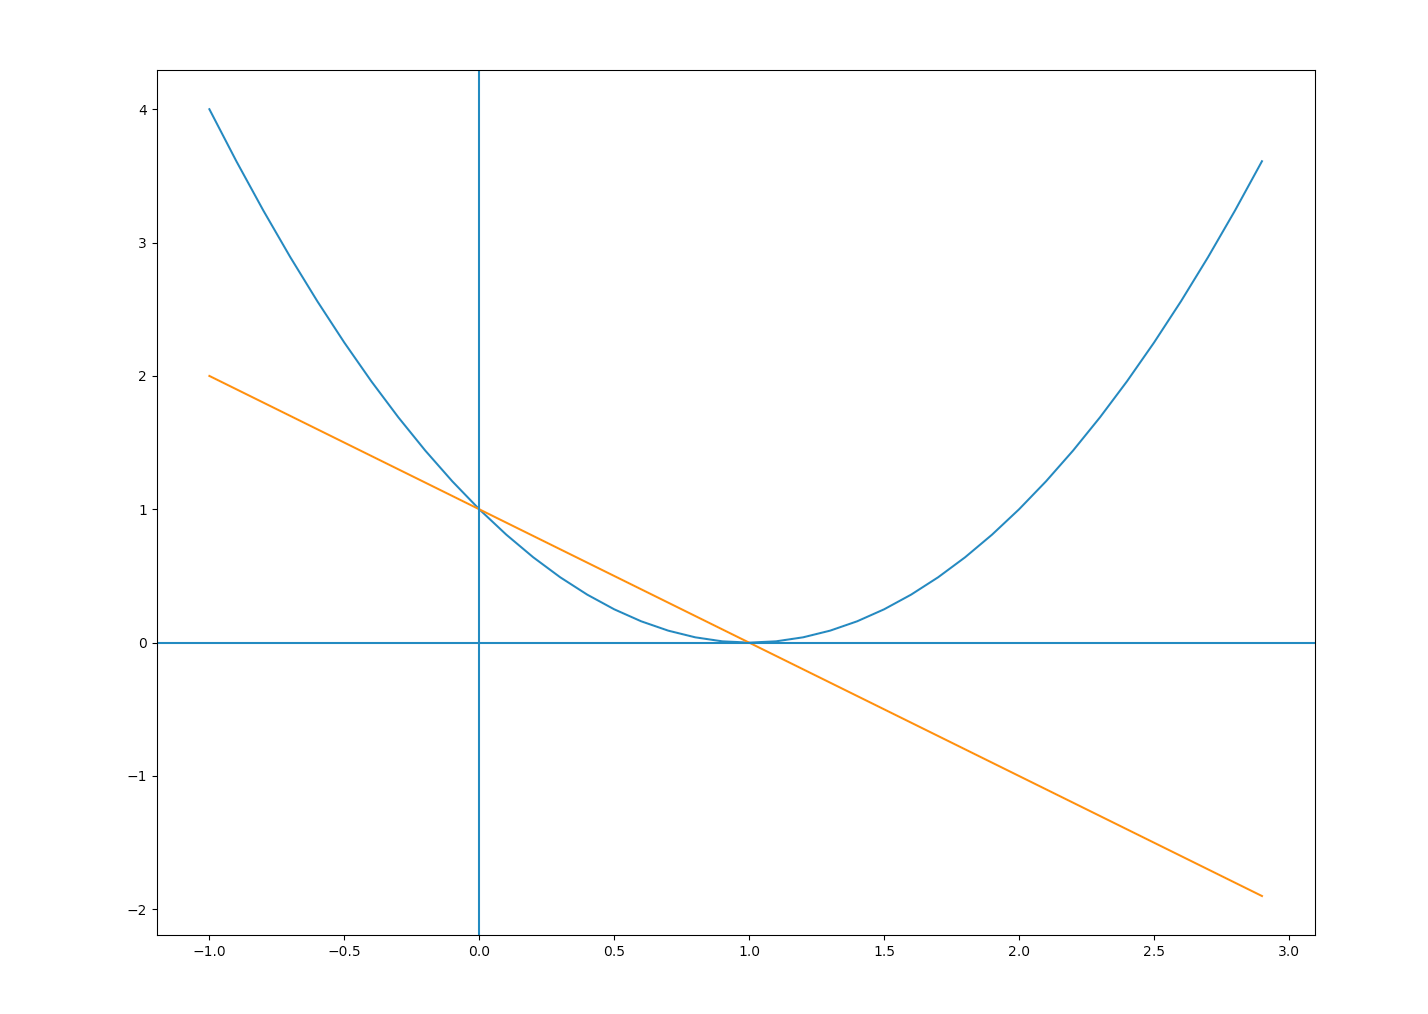
\includegraphics[height=3cm]{Figure_1}}
  \end{itemize}
\end{frame}

\begin{frame}
  \frametitle{LPI - Example (cont)}
  \begin{itemize}
  \item Lets add an additional data point (-1, 4)
    \[
      \begin{array}{ll}
        x_0 = 0 & a_0 = 1 \\
        x_1 = 1 & a_1 = 0 \\
        x_2 = -1& a_2 = 4 \\
      \end{array}
    \]
    So    
    \[
      \begin{array}{lll}
        L_0(x) & = & \frac{x-x_1}{x_0-x_1} \frac{x - x_2}{x_0-x_2} = -(x-1)(x+1)\\
        L_1(x) & = & \frac{x-x_0}{x_1-x_0} \frac{x - x_2}{x_1-x_2} = \mbox{Don't care}\\
        L_2(x) & = & \frac{x-x_0}{x_2-x_0} \frac{x - x_1}{x_2-x_1} = \frac{1}{2} x (x-1)\\
      \end{array}
    \]
  \end{itemize}
\end{frame}

\begin{frame}
  \frametitle{LPI - Example (cont)}
  \begin{itemize}
  \item Putting it all together
    \[
      \begin{array}{lll}
        p(x) & = & a_0 L_0(x) + a_1 L_1(x) + a_2 L_2(x)\\
             & = & -(x-1)(x+1) + 2 x (x-1) \\
             & = & (x-1) ( -x - 1 + 2x)\\
             & = & (x-1) (x-1) = (x-1)^2\\
      \end{array}
    \] \pause
    \item The approximation is exact
    \item For large data-sets Lagrange can be a challenge
    \item Meandering between data-points can become significant
  \end{itemize}
\end{frame}

\section{Cubic Spline Interpolation}

\begin{frame}
  \frametitle{Cubic spline interpolation}
  \begin{itemize}
  \item Smoothing w.\ constraints 
  \item Limiting higher order gradients (say acceleration, curvature, ...)
    \[
      \begin{array}{lll}
        f'''' & = & 0\\
        f'''  & = & c_1\\
        f''   & = & c_1 x + c_2\\
        f'    & = & \frac{c_1}{2} x^2 + c_2 x + c_ 3\\
        f     & = & \frac{c_1}{6} x^3 + \frac{c_2}{2} x^2 + c_3 x + c_4\\                    
      \end{array}
    \]
  \end{itemize}
\end{frame}
\begin{frame}
  \frametitle{Setting it up}
  \begin{itemize}
  \item Assume you have tabulated values $y_i = y(x_i)$ for $i = 0 \ldots n-1$
  \item With linear interpolation we can do
    \[
      y = A y_j + B y_{j+1}
    \] for a point between $x_j$ and $x_{j+1}$ where
    \[
      \begin{array}{ll}
        A = \frac{x_{j+1} - x}{x_{j+1}-x_j} & B = 1-A = \frac{x - x_j}{x_{j+1} - x_j}
      \end{array}
    \] so think of them as special cases of Lagrange
  \item if we further assume we have access to values of $y''$ we can do a cubic expansion
  \end{itemize}
\end{frame}

\begin{frame}
  \frametitle{Cubic interpolation}
  \begin{itemize}
  \item We can expand the interpolation
    \[
      y = A y_j + B y_{j+1} + C y^{''}_j + D y^{''}_{j+1}
    \]
    where A and B are as defined earlier.
    \[
      \begin{array}{cc}
        C = \frac{1}{6} (A^3-A)(x_{j+1} - x_j)^2 ~~~ & ~~~
        D = \frac{1}{6} (B^3-B)(x_{j+1} - x_j)^2\\                                                       
      \end{array}
    \]
  \item If you differentiate (see NR sec 3.3) you get
    \[
      \frac{d^2y}{dx^2} = A y^{''}_j + B y^{''}_{j+1}
    \]
    which translate into the tabulated values at $x_j$ and $x_{j+1}$.
  \item The advantage of cubic is that only neighboring points are
    used in estimation. A tridiagonal matrix can be used for the
    computations. 
  \end{itemize}
\end{frame}

\section{Multi-variate interpolation}

\begin{frame}
  \frametitle{What about multi-variate interpolation? }
  \begin{itemize}
  \item Does this generalize to multiple dimensions? 
  \item We frequently have multi-dimensional data in robotics
    \begin{itemize}
    \item Image data, Lidar, radar, ...
    \end{itemize}
  \item What if we had an m-dimensional Cartesian mesh of data points?
    \[
      f(\vec{x}) = f(x_{1i}, x_{2j}, x_{3k}, \ldots, x_{mq})
    \]
  \item For linear interpolation the generalization is straight forward
  \end{itemize}
\end{frame}

\begin{frame}
  \frametitle{Bilinear interpolation}
  \begin{itemize}
  \item Consider
    \[ y_{ij} = y(x _{1i}, x_{2j}) \]
  \item with point intervals [$x_{1i}, x_{1(i+1)}$] and  [$x_{2j}, x_{2(j+1)}$] 
  \item values for ij
    \[
      \begin{array}{ccc}
        y_0& = & y_{ij}\\
        y_1& = & y_{(i+1)j}\\
        y_2& = & y_{(i+1)(j+1)}\\
        y_3& = & y_{i(j+1)}\\
      \end{array}
    \]
  \end{itemize}
\end{frame}

\begin{frame}
  \frametitle{Bilinear interpolation (cont)}
  \begin{itemize}
  \item The bilinear interpolation is the simplest
  \item use
    \[
      \begin{array}{ccc}
        t & = & \frac{x_1 - x_{1i}}{x_{1(i+1)} - x_{1i}}\\
        u & = & \frac{x_2 - x_{2j}}{x_{2(j+1)} - x_{2j}}\\
      \end{array}
    \]
  \item then the interpolation is:
    \[
      y(x_1, x_2) = (1-t)(1-u) y_0 + t(1-u) y_1 + tu y_2 + (1-t)u y_3
    \]
  \item For a fair sized grid this generates ``good'' solutions. 
  \end{itemize}
\end{frame}

\section{Kringing Interpolation}

\begin{frame}
  \frametitle{Kringing interpolation}
  \begin{itemize}
  \item What if we consider the data generation by a stochastic process? 
  \item Could we generate a maximum likelihood (ML) estimate?
  \item The data is a vector of samples from the process and we can
    compute the probability density estimate and parameters such as
    the mean
  \item Sometimes termed Gaussian Process Regression
  \item More generally we are trying to estimate
    \[
      f(x) = \sum_{i=0}^N w_i \phi_i(x) = \vec{w} \Phi(\vec{x})
    \]
    where w are weights and $\phi$ is a basis function.
    \pause
  \item We can define a loss function
    \[ L(f, y) \]
  \item The expected loss is then
    \[ E[L] = \int \int L( f, y(x) ) p(x,w) dx dw \]
  \item Our goal is now to minimize the $E[L]$, i.e. minimum loss or best fit
    \[ f = E(y|x) \]
  \end{itemize}
\end{frame}

\begin{frame}
  \frametitle{Basis functions}
  \begin{itemize}
  \item We have multiple choices for basis functions
  \item Sometimes domain knowledge can provide suggestions
  \item Polynomial basis functions
    \[ \phi_i(x) = x_i \]
  \item Gaussian basis functions
    \[
      \phi_i(x) = e^{-\frac{(x-x_i)^2}{2s}}
    \]
    $s$ controls scale / coverage
  \item Sigmoid basis functions
    \[
      \phi_i(x) = \sigma \left( \frac{ x-x_i }{s} \right)
    \] where
    $\sigma(a) = \frac{1}{1+e^{-a}}$
  \end{itemize}
\end{frame}

\begin{frame}
  \frametitle{Kringing interpolation - Gaussian Mixture}
  \begin{itemize}
  \item For the Gaussian mixture we can use
    \[ p(f_i | x_i, w_i, \beta) = N( f_i | y(x_i), w_i, \beta)  \]
  \item so that
    \[
      p( f | X, w, \beta) = \prod_{i=0}^n N(f_i | w^T \phi(x_i), \beta^{-1})
    \] or
    \[
      ln p() = \frac{n}{2} ln(\beta)  - \frac{n}{2} ln(2\pi) - \beta E_D(w)
    \] where
    \[ E_D(w) = \frac{1}{2} \sum_{i=0}^n (y_i - w^T_i \phi(x_i))^2 \] The sum of squared errors
  \end{itemize}
\end{frame}

\begin{frame}
  \frametitle{LSQ solution}
  \begin{itemize}
  \item We can compute
    \[
      w_{ML} = (\Phi^T \Phi)^{-1} \Phi^T \vec{y}
    \]
    where
    \[
      \Phi = \left(
        \begin{array}{cccc}
          \phi_1(x_1) & \phi_2(x_1) & \ldots & \phi_n(x_1) \\
          \phi_1(x_2) & \phi_2(x_2) & \ldots & \phi_n(x_2) \\
                      & \vdots      &        &             \\
          \phi_1(x_n) & \phi_2(x_n) & \ldots & \phi_n(x_n) \\
        \end{array} \right)
      \]
  \end{itemize}
\end{frame}

\begin{frame}
  \frametitle{Kringing example}
  \begin{center}
      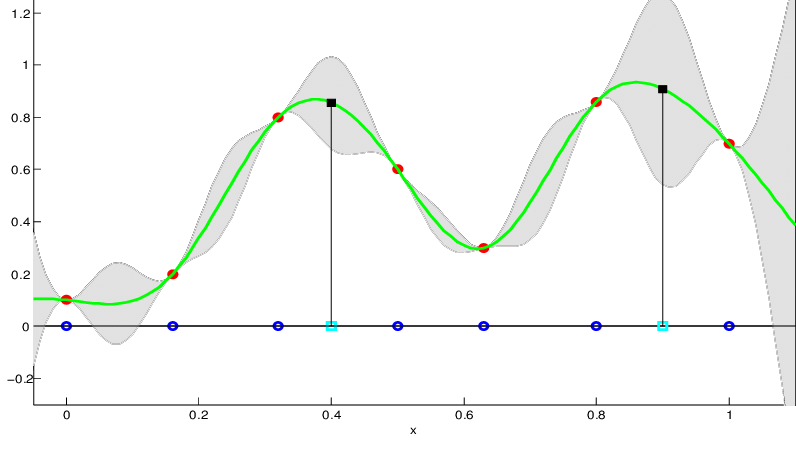
\includegraphics[width=9cm]{kringing-1d-example}
  \end{center}
\end{frame}

\begin{frame}
  \frametitle{Regularized Kringing}
  \begin{itemize}
  \item We can use a regularized LSQ if we want to control the variation in w. 
  \item Consider a revised error function
    \[ E' = E_D(w) + \lambda E_w(w) \] say
    \[ E' = \frac{1}{2} \sum_i (y_i - w^T\phi(x_i))^2 + \frac{\lambda}{2} w^T w \]
    which is minimized by
    \[
      w = (\lambda + \Phi^T \Phi)^{-1} \Phi^T \vec{y}
    \]
    as an example of how you can tweak the optimization / approximation    
  \end{itemize}
\end{frame}


\section{Summary}

\begin{frame}
  \frametitle{Summary}
  \begin{itemize}
  \item Model based and data driven interpolation / approximation
  \item Basic Methods (Linear)
  \item Spline based interpolation
  \item Uni- and Multi-Variate Approaches
  \item Stochastic Models
  \item Next time functional interpolation \& approximation 
  \end{itemize}
\end{frame}
\end{document}

%%% Local Variables:
%%% mode: latex
%%% TeX-master: t
%%% End:
